% elementos pós-textuais 
\postextual

%% apêndice 
%\begin{apendicesenv}
%\partapendices
%
%\chapter{PRIMEIRO APÊNDICE}
%
%\lipsum[50]
%
%\chapter{SEGUNDO APÊNDICE}
%
%\lipsum[50]
%
%\end{apendicesenv}

% anexos 
\begin{anexosenv}
\partanexos

\chapter{código para construção da base de dados}\label{anexo_a}

\begin{lstlisting}[frame=single]
  # pacotes
  library(magrittr, include.only = "%>%")
  
  # municípios x regiões imediatas
  municipios = basedosdados::read_sql("
  SELECT
    id_municipio
    , nome
    , nome_mesorregiao
    , nome_microrregiao
    , nome_regiao
    , nome_regiao_imediata
    , nome_regiao_intermediaria
  FROM `basedosdados.br_bd_diretorios_brasil.municipio`
  WHERE sigla_uf = 'ES'
  ")
  
  # estban
  estban = basedosdados::read_sql("
  SELECT
    CAST(ano AS STRING) AS ano
    , CAST(mes AS STRING) AS mes
    , id_municipio
    , cnpj_agencia
    , CASE
          WHEN id_verbete = '160' THEN 'operações de crédito'
          WHEN id_verbete = '161' THEN 'empréstimos e títulos descontados'
          WHEN id_verbete = '162' THEN 'financiamentos'
          WHEN id_verbete = '163' THEN 'financiamentos rurais'
          WHEN id_verbete = '169' THEN 'financiamentos imobiliários'
          WHEN id_verbete = '172' THEN 'outros créditos'
          WHEN id_verbete = '174' THEN 'provisão para operações de crédito'
          ELSE 'outros'
      END AS verbete
    , valor
  
  FROM `basedosdados.br_bcb_estban.agencia`
  
  WHERE
    -- CNPJ do Banestes
    cnpj_basico = '28127603'
    -- filtrando verbetes de interesse
    AND id_verbete IN ('161', '162', '163', '169')
  ")
  
  # formatando datas
  estban = within(estban, {
    mes = formatC(as.numeric(mes), format = "d", width = 2, flag = "0")
    ref = as.Date(paste(ano, mes, "01", sep = "-"))
  })
  
  # identificando agências em atividade
  agencias_fim = subset(estban, ref == max(ref), select = cnpj_agencia) |>
    (\(x) unique(x$cnpj_agencia))()
  
  # filtrando apenas agências em atividade
  estban = subset(
    estban,
    cnpj_agencia %in% agencias_fim
  )

  # mesclando com tabela municípios
  estban = merge(estban, municipios, by = "id_municipio")

\end{lstlisting}

\begin{figure}[h]
  \caption{Modelo de dados}
  \label{fig-data_model}
  \begin{center}
    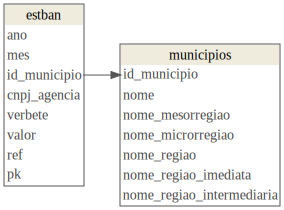
\includegraphics[width=8cm]{img/data_model.png}
  \end{center}
\end{figure}

\end{anexosenv}

% índice remissivo 
\phantompart
\printindex
